\documentclass{article}
\usepackage{graphicx}
\usepackage{subfigure}
\usepackage{caption}
\usepackage{lipsum}
\usepackage{amsmath}
\usepackage{amsthm}
\usepackage{geometry}
\usepackage{amsfonts}
\usepackage{ragged2e}
\usepackage{amssymb}
\usepackage{mathrsfs}
\usepackage{enumitem}
\geometry{
 a4paper,
 total={170mm,257mm},
 left=20mm,
 top=20mm,
 }
\usepackage[utf8]{inputenc}

\title{Tarea 2 Metodos Computacionales}
\author{Luis Mantilla}
\date{July 2019}

\begin{document}

\maketitle

\section*{Punto 1}

La idea de este ejercicio es lograr unir dos im\'agenes de tal manera que vista desde cerca sea una imagen y vista desde lejos sea la otra imagen. Esto lo podemos hacer tomando el espectro de Fourier de ambas im\'agenes y tomar las frecuencias altas de una y las bajas de otra y finalmente sumar ambas.


Las dos im\'agenes que vamos a unir son las siguientes:
\begin{figure}[!htbp]
  \centering
  \subfigure[Seria]{
    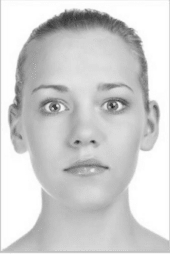
\includegraphics[width=0.23\textwidth]{cara_02_grisesMF.png}%
    }\hspace{0.2cm}
    \subfigure[Sonriendo]{
    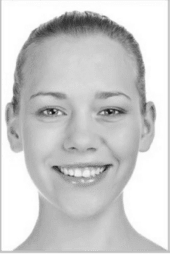
\includegraphics[width=0.228\textwidth]{cara_03_grisesMF.png}%
  }  
  \caption{Caras a unir}
\end{figure}


La transformada de Fourier de cada imagen es la siguiente:
\begin{figure}[!htbp]
 \centering
  \includegraphics[scale=0.5]{TransformadaAmbasCaras.png}
\end{figure}

Podemos filtrar con una función Sigmond para obtener una funci\'on escal\'on suavizada
\begin{equation*}
    f(x) = \frac{1}{1+ \exp(-15x)}
\end{equation*}

Despues del filtrado tendremos las siguentes caras:
\begin{figure}[!htbp]
  \centering
  \subfigure[Seria]{
    \includegraphics[width=0.53\textwidth]{CaraPasaAltas.png}%
    }\hspace{0.05cm}
    \subfigure[Sonriendo]{
    \includegraphics[width=0.528\textwidth]{CaraPasaBajas.png}%
  }  
  \caption{Caras despues del filtrado}
\end{figure}


La transformada de Fourier de ambas despu\'es del filtro es
\begin{figure}[!htbp]
 \centering
  \includegraphics[scale=0.6]{TransformadaHibrida.png}
\end{figure}

El resultado final que obtenemos de ambas im\'agenes es

\begin{figure}[!htbp]
 \centering
  \includegraphics[scale=0.6]{CaraHibrida.png}
  \caption{De cerca se ve una cara seria y de lejos una cara sonriendo}
\end{figure}

\pagebreak

\section*{Punto 2}

En este ejercicio buscamos solucionar la ecuaci\'on diferencial de segundo orden de la fuerza gravitacional entre dos masas.
\begin{equation*}
    \frac{d^2 \Vec{r}}{dt^2} = \frac{GMm }{r^2} \hat{r}
\end{equation*}

Esto lo podemos descomponer en dos ecuaciones de primer orden para poder solucionarlas simult\'aneamente

\begin{equation*}
    \frac{d \Vec{v}}{dt} = \frac{GMm }{r^2} \hat{r}
\end{equation*}

y

\begin{equation*}
    \frac{d\Vec{r}}{dt} = \Vec{v}
\end{equation*}

Solucionamos las siguentes ecuaciones con distintas elecciones de dt para aproximar las derivadas temporales. Se hace con 3 distintos valores de dt. 
\begin{itemize}
    \item $dt1=0.0006283 $[YR]
    \item $dt2 = 0.006283$ [YR]
    \item $dt3 = 0.12566$ [YR]
\end{itemize}
\begin{figure}[!htbp]
 \centering
  \includegraphics[width=1\textwidth]{posiciones.png}
\end{figure}

Dado que estamos trabajando con unidades de Unidades Astron\'omicas [AU], Masas Solares [MS] y a\~nos [YR], los valores de energ\'ias cin\'eticas, potenciales, totales y los momentos angulares los multipliqu\'e por un factor de $100000$ para notar las fluctuaciones en las gr\'aficas.

Se puede apreciar que el m\'etodo de Euler es el que peor simula esta situaci\'on dado a la forma como aproxima (con forward difference) y el que mejor simula es RungeKutta (aunque LeapFrog tambi\'en hace un muy buen trabajo)

\begin{figure}[!htbp]
 \centering
  \includegraphics[width=1\textwidth]{angularMomentum.png}
  \caption{Momento Angular}
\end{figure}

\begin{figure}[!htbp]
 \centering
  \includegraphics[width=1\textwidth]{EnergiaPotencial.png}
  \caption{Energia Potencial}
\end{figure}

\begin{figure}[!htbp]
 \centering
  \includegraphics[width=1\textwidth]{EnergiaCinetica.png}
  \caption{Energia Cinetica}
\end{figure}

\begin{figure}[!htbp]
 \centering
  \includegraphics[width=1\textwidth]{EnergiaTotal.png}
  \caption{Energia Total (Cinetica + Potencial)}
\end{figure}

Vemos que la energ\'ia total pr\'acticamente se conserva cuando implementamos el m\'etodo de RungeKutta y LeapFrog, se mantienen muy estables. En contraste, el m\'etodo de Euler presenta grandes fallos, y la energ\'ia no se esta conservando, aumenta en cada paso. En el caso de la energ\'ia cin\'etica y la energ\'ia potencial, es claro ver que comienzan y terminan en puntos opuestos y presentan comportamientos peri\'odicos, de tal manera que la suma es constante. Este comportamiento peri\'odico ocurre cuando la tierra esta en el Perihelio o en el Afelio.





\end{document}

